%---------------------------------------------------------------%
%-------------- MODELO DE DISSERTAÇÃO PROFMAT/UFT --------------%
%---------------------------------------------------------------%

\documentclass[
  % -- opções da classe memoir --
  12pt,                 % Tamanho da fonte
  openright,            % Capítulo começa em pág ímpar (insere página vazia se preciso)
  oneside,              % Impressão em frente. Oposto a twoside
  a4paper,              % Tamanho do papel 
  % -- opções da classe abntex2 --
  chapter=TITLE,        % Títulos de capítulos em letras maiúsculas
  % -- opções do pacote babel --
  english,              % Idioma adicional para hifenização
  brazil,               % Último idioma é o principal do documento
  ]{abntex2}

% ---
% Customizações para adequação do modelo às normas ABNT e ao Manual de Normalização para Elaboração de Trabalhos Acadêmico-Científicos da UFT
% ---
% Pacotes Principais
% ---
\usepackage[left=3cm,right=2cm,top=3cm,bottom=2cm]{geometry}    % layout de página
\usepackage{lmodern}		% Usa a fonte Latin Modern
\usepackage[T1]{fontenc}	% Selecao de codigos de fonte.
\usepackage[utf8]{inputenc}	% Codificacao do documento (conversão automática dos acentos)
\usepackage{indentfirst}	% Indenta o primeiro parágrafo de cada seção.
\usepackage{color}			% Controle das cores
\usepackage{graphicx}		% Inclusão de gráficos
\usepackage{microtype} 		% para melhorias de justificação
\usepackage{pslatex}        % torna o documento padrão para as fontes Times/Helvetica/Courier
\usepackage{url}
\usepackage{booktabs}
\usepackage{subfig}
\usepackage{pdfpages}
\usepackage{lastpage}
\usepackage{fancyhdr}
\usepackage{float}
\usepackage{caption}
\usepackage{amsmath, amssymb, amsthm, amsfonts}
\usepackage{setspace}
\usepackage{chngcntr}
\usepackage{keystroke}
\usepackage{tocloft}
\usepackage{longtable, ltcaption}
\usepackage{newfloat}
\usepackage{tikz}
% ---
% ---
% Pacote de citações
% ---
\usepackage[alf,abnt-etal-text=it,abnt-repeated-author-omit=yes,abnt-etal-list=0,abnt-etal-cite=4,abnt-emphasize=bf]{abntex2cite}
% ---


% ---
% Customizações de Fontes e Tamanhos de Letras usados na Classe ABNTEX2
% ---
\renewcommand{\chaptitlefont}{\ABNTEXchapterfont\ABNTEXchapterfontsize}

\setsecheadstyle{\ABNTEXsectionfont\ABNTEXsectionfontsize\ABNTEXsectionupperifneeded}

\renewcommand{\ABNTEXchapterfont}{\rmfamily}
\renewcommand{\ABNTEXchapterfontsize}{\normalsize\bfseries}

\renewcommand{\ABNTEXpartfont}{\ABNTEXchapterfont}
\renewcommand{\ABNTEXpartfontsize}{\LARGE\bfseries}
\renewcommand{\cftpartfont}{\normalfont\rmfamily\bfseries}
\renewcommand{\cftpartpagefont}{\normalfont\rmfamily\bfseries}

\renewcommand{\ABNTEXsectionfont}{\ABNTEXchapterfont}
\renewcommand{\ABNTEXsectionfontsize}{\bfseries}

\renewcommand{\ABNTEXsubsectionfont}{\ABNTEXsectionfont}
\renewcommand{\ABNTEXsubsectionfontsize}{\normalsize}

\renewcommand{\ABNTEXsubsubsectionfont}{\ABNTEXsubsectionfont}
\renewcommand{\ABNTEXsubsubsectionfontsize}{\normalsize}

\renewcommand{\ABNTEXsubsubsubsectionfont}{\ABNTEXsubsectionfont}
\renewcommand{\ABNTEXsubsubsubsectionfontsize}{\normalsize}
% ---

% ---
% Customização do Sumário (Distância entre número e nome do item)
% ---
\setlength{\cftlastnumwidth}{3.5em}
\cftsetindents{part}{0em}{\cftlastnumwidth}
\cftsetindents{chapter}{0em}{\cftlastnumwidth}
\cftsetindents{section}{0em}{\cftlastnumwidth}
\cftsetindents{subsection}{0em}{\cftlastnumwidth}
\cftsetindents{subsubsection}{0em}{\cftlastnumwidth}
\cftsetindents{paragraph}{0em}{\cftlastnumwidth}
\cftsetindents{subparagraph}{0em}{\cftlastnumwidth}

% ---
% Possibilita criação de Quadros e Lista de quadros.
% Ver https://github.com/abntex/abntex2/issues/176
%
\renewcommand{\insertchapterspace}{}
\newcommand{\listofquadrosname}{}
\DeclareFloatingEnvironment[
    fileext=loq,
    listname={Lista de Quadros},
    name=Quadro,
    placement=p,
    within=none,
    chapterlistsgaps=off,
    ]{quadro}

\newlistof{listofquadros}{loq}{\listofquadrosname}
\newlistentry{quadro}{loq}{0}

% configurações para atender às regras da ABNT
\setfloatadjustment{quadro}{\centering}
\counterwithout{quadro}{chapter}
\renewcommand{\cftquadroname}{\quadroname\space} 
\renewcommand*{\cftquadroaftersnum}{\hfill--\hfill}


\setfloatlocations{quadro}{hbtp} % Ver https://github.com/abntex/abntex2/issues/176
% ---

\setlength{\cftbeforechapterskip}{0pt} % Altera o espaçamento entre itens do sumário
% ---

% ---
% Customizações Adicionais
% ---
\providecommand{\imprimircampus}{}
\newcommand{\campus}[1]{\renewcommand{\imprimircampus}{#1}}

\providecommand{\imprimirsubtitulo}{}
\newcommand{\subtitulo}[1]{\renewcommand{\imprimirsubtitulo}{#1}}

\providecommand{\imprimirexaminadorA}{}
\newcommand{\examinadorA}[1]{\renewcommand{\imprimirexaminadorA}{#1}}

\providecommand{\imprimirexaminadorB}{}
\newcommand{\examinadorB}[1]{\renewcommand{\imprimirexaminadorB}{#1}}

\counterwithout{equation}{chapter} % define uma numeração contínua (1,2,3, ...) de equações. Para uma numeração com dependência do número do capítulo (1.1, 1.2, ...), basta apagar esta linha.

\setlength{\ABNTEXsignwidth}{10cm} % define o comprimento da linha de assinatura na folha de aprovação

\setlength{\ABNTEXsignthickness}{0.5pt} % define a espessura da linha de assinatura na folha de aprovação

% Redefine o ambiente citacao para que as citações diretas com mais de 3 linhas tenham recuo de 4 cm
\renewenvironment{citacao}[1][default]{%
   \list{}{\leftmargin=0cm}%
   \ABNTEXfontereduzida%
   \addtolength{\leftskip}{\ABNTEXcitacaorecuo}%
   \item[]%
   \begin{SingleSpace}%
   \ifthenelse{\not\equal{#1}{default}}{\itshape\selectlanguage{#1}}{}%
 }{%
   \end{SingleSpace}%
   \endlist}%


% O tamanho do parágrafo é dado por:
\setlength{\parindent}{1.25cm}

%\setlength{\parskip}{0.2cm}  % tente também \onelineskip

% Controle do espaçamento entre um parágrafo e outro:
\setlength{\cftparskip}{0pt}

%\renewcommand{\baselinestretch}{1.5}
\linespread{1.5}

% Altera o aspecto da cor azul
\definecolor{blue}{RGB}{41,5,195}
% ---

% informações do PDF
\makeatletter
\hypersetup{
     	%pagebackref=true,
		pdftitle={\@title}, 
		pdfauthor={\@author},
    	pdfsubject={\imprimirpreambulo},
	    pdfcreator={LaTeX with abnTeX2},
		pdfkeywords={abnt}{latex}{abntex}{abntex2}{projeto de pesquisa}, 
		colorlinks=true,       		% false: boxed links; true: colored links
    	linkcolor=black,          	% color of internal links
    	citecolor=black,        		% color of links to bibliography
    	filecolor=black,      		% color of file links
		urlcolor=black,
		bookmarksdepth=4
}
\makeatother
% --- 

% ---
% Modelo de Capa conforme Manual UFT
\renewcommand{\imprimircapa}{
\begin{capa}
    \begin{center}
    	
\includegraphics[scale=0.12]{img/brasao.png}\\
 		\MakeUppercase{\textbf{\imprimirinstituicao}}\\
 		\MakeUppercase{\textbf{CÂMPUS UNIVERSITÁRIO DE \imprimircampus}}\\
 		\textbf{PROGRAMA DE MESTRADO PROFISSIONAL EM MATEMÁTICA\\ EM REDE NACIONAL -- PROFMAT}\\
 		\vspace{2.5cm}
		\MakeUppercase{\textbf{\imprimirautor}}\\
        \vspace{3.5cm}
        \MakeUppercase{\textbf{\imprimirtitulo}}\\
        \MakeUppercase{\imprimirsubtitulo}
        \vfill
        \MakeUppercase{\imprimircampus} (TO)\\
        \imprimirdata
    \end{center}
\end{capa}
}
% ---

% ---
% Modelo de Folha de Rosto conforme Manual UFT
\renewcommand{\imprimirfolhaderosto}{
\begin{folhaderosto}
    \begin{center}
     	\MakeUppercase{\textbf{\imprimirautor}}\\
     	\vspace{5cm}
     	\MakeUppercase{\textbf{\imprimirtitulo}} \\
     	\MakeUppercase{\imprimirsubtitulo}
     \end{center}
     \vspace{3.5cm}
     \hspace{8cm}
        \begin{minipage}{8cm}
			\SingleSpacing
			\imprimirpreambulo
		\end{minipage}\\
	\begin{center}
        \vfill
        \MakeUppercase{\imprimircampus} (TO) \\
        \imprimirdata
    \end{center}
\end{folhaderosto}
}
% ---
% ---

% ---
% Compila o índice
% ---
\makeindex
% ---

% ---
% Abra o arquivo dados_academicos.tex e preencha os dados referentes ao trabalho (autor, título, orientador, etc.)
% ---
% Informações do Trabalho a serem informadas pelo AUTOR
% ---
\titulo{Título do Trabalho Acadêmico}

\subtitulo{Subtítulo do Trabalho Acadêmico (Se Houver)}   
% Caso não haja subtítulo, basta apagar esta linha.

\autor{Nome do Autor}

\orientador{Prof. Dr. ``Nome do Orientador''}

\instituicao{Universidade Federal do Tocantins}

\campus{Palmas}

\data{20XX}

\tipotrabalho{Dissertação (Mestrado)}

% O preambulo deve conter o tipo do trabalho, o objetivo, 
% o nome da instituição e a área de concentração 
\preambulo{Dissertação apresentada ao Programa de Mestrado Profissional em Matemática em Rede Nacional - PROFMAT da Universidade Federal do Tocantins como requisito parcial para a obtenção do título de Mestre - Área de Concentração: Matemática.\\
Orientador: \imprimirorientador.}
% ---
% --- 

%---------------------------------------------------------------%
%--------------------------DISSERTAÇÃO--------------------------%
%---------------------------------------------------------------%

\begin{document}
\DeclareGraphicsExtensions{.jpg,.pdf,.eps,.png}

% Retira espaço extra obsoleto entre as frases.
\frenchspacing


%--------------------ELEMENTOS PRÉ-TEXTUAIS--------------------%

% Abra o arquivo pretextual.tex para alterar os elementos pré-textuais de seu trabalho 

%--------------------ELEMENTOS PRÉ-TEXTUAIS--------------------%

%-----------------------------Capa-----------------------------%
\imprimircapa


%------------------------Folha de rosto------------------------%
\imprimirfolhaderosto


%----------------------Ficha Catalográfica----------------------%

% Após a aprovação do trabalho, acesse o link: https://sistemas.uft.edu.br/ficha/

% No formulário do site, preencha os campos desses elementos com os dados do trabalho acadêmico. 
% O programa fará a ordenação e formatação correta dos dados, apresentando a ficha finalizada e normalizada. 
% Faça o download da ficha em formato PDF e salve-a com o nome: ficha_catalografica.pdf
% Substitua o arquivo temporário de mesmo nome presente neste modelo.

\begin{fichacatalografica}
    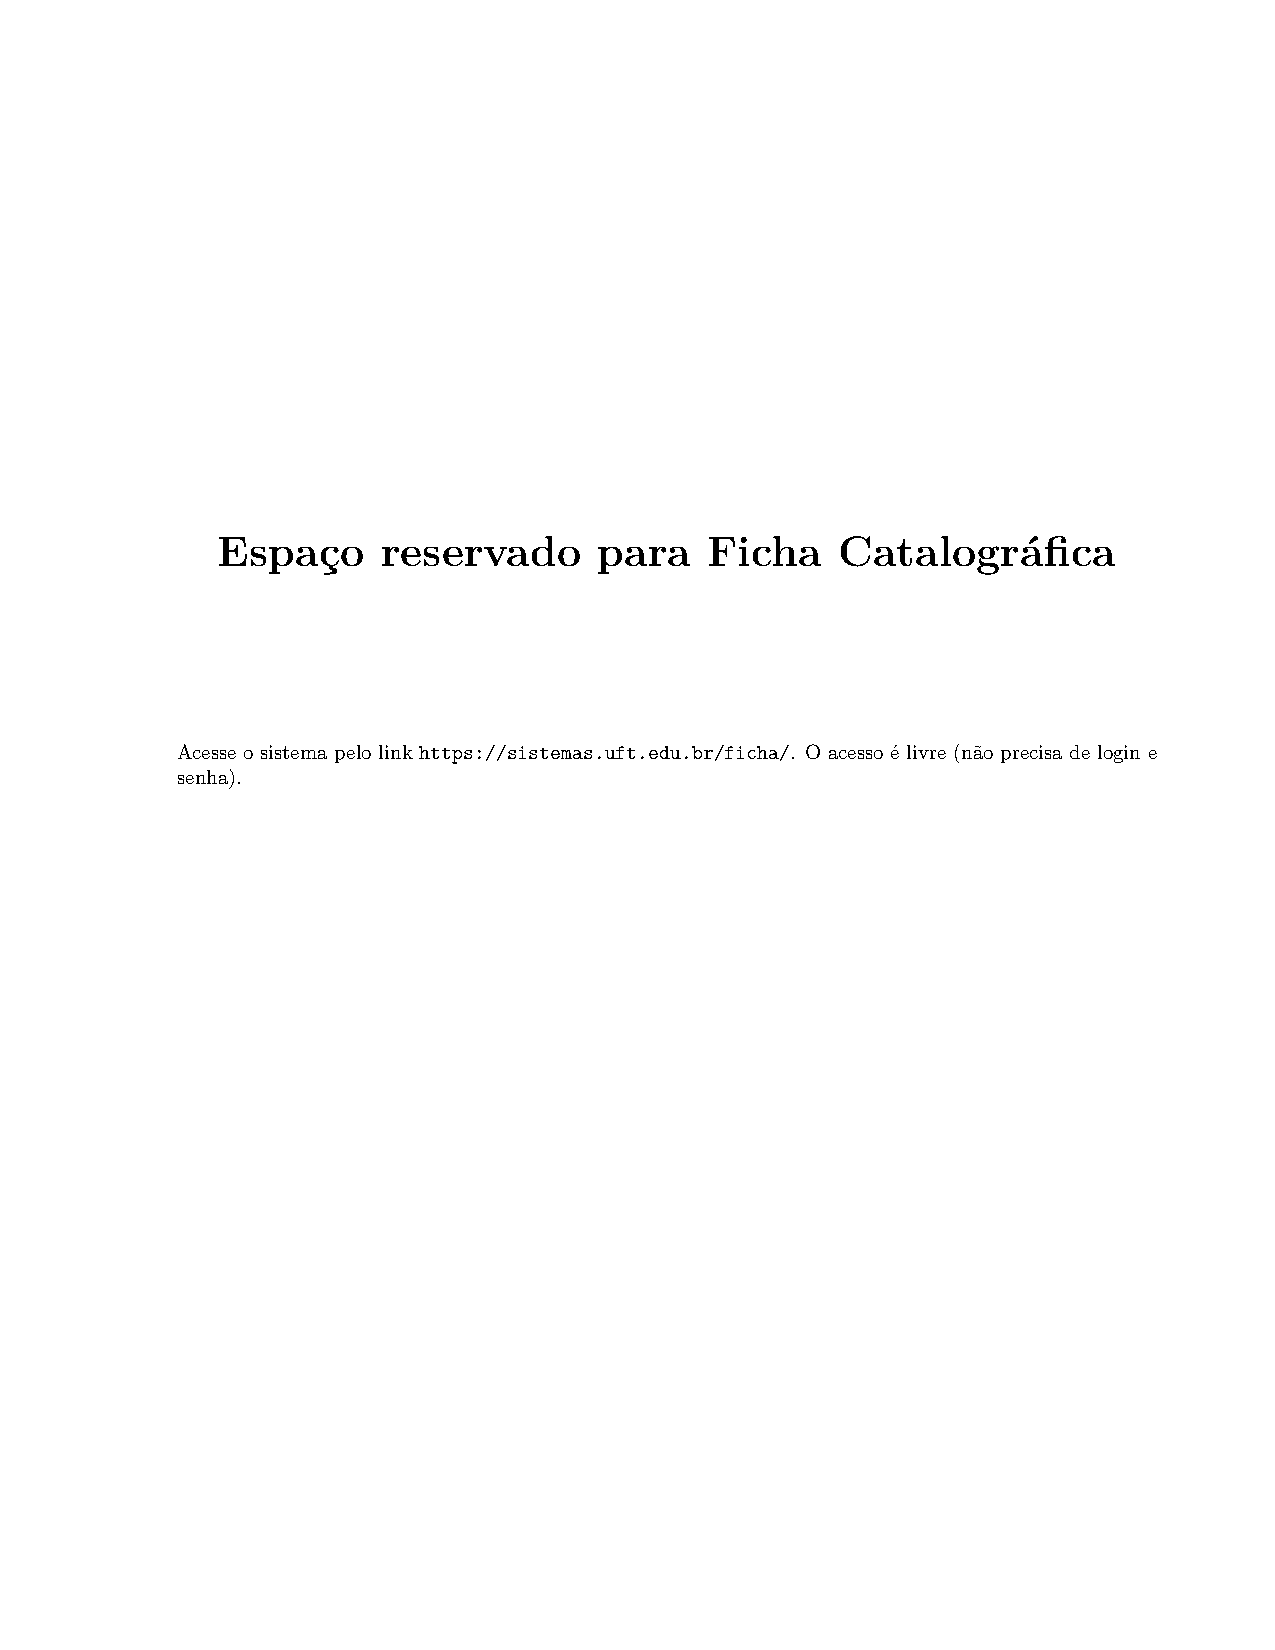
\includepdf{ficha_catalografica.pdf}
\end{fichacatalografica}


%----------------------Folha de Aprovação----------------------%

% Após aprovação do trabalho, solicite do orientador a Folha de Aprovação assinada pela Banca Examinadora.
% Salve-a em formato PDF com o nome: folha_aprovacao.pdf
% Substitua o arquivo temporário de mesmo nome presente neste modelo.

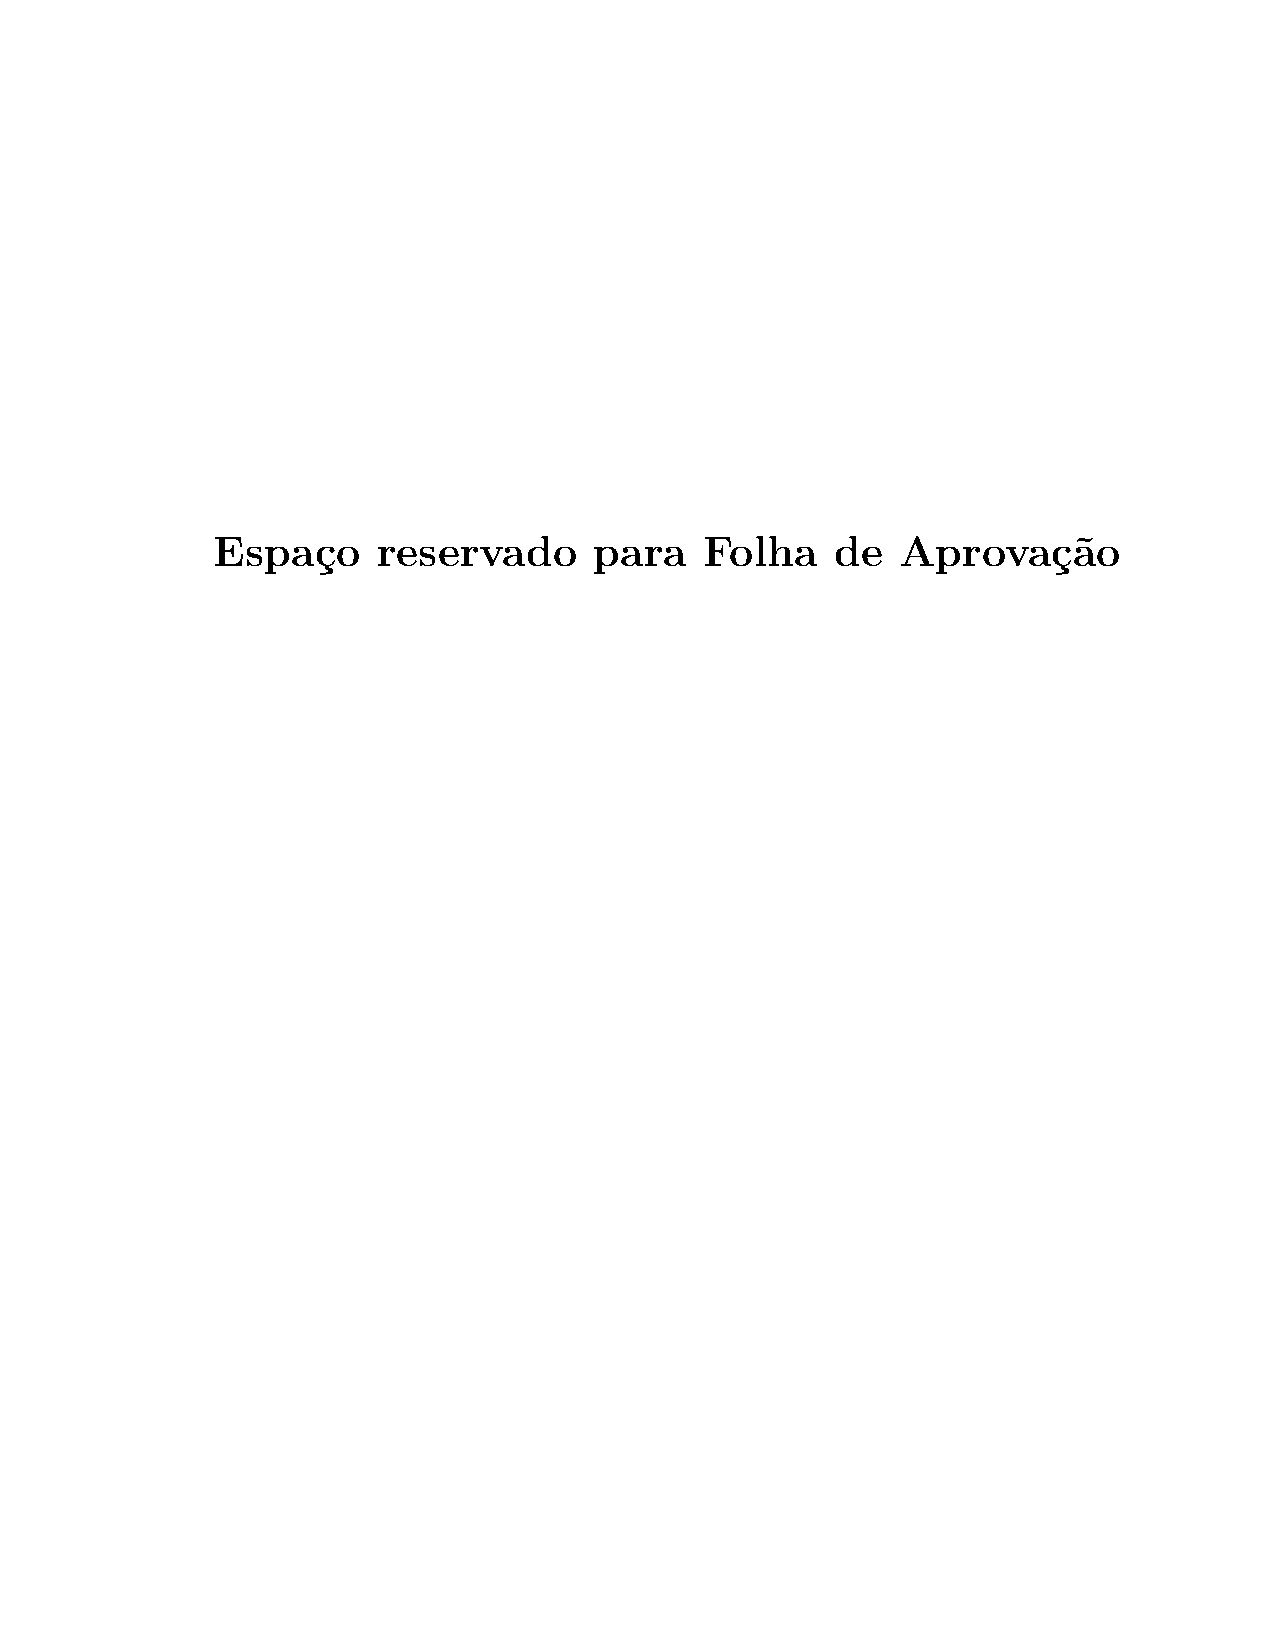
\includepdf{folha_aprovacao.pdf}


%----------------------Dedicatória----------------------%
\begin{dedicatoria}
\vspace*{\fill}
	\begin{flushright}
		\textit{
            A Fulano.\\
   		   A Beltrano.
        }
	\end{flushright}
\end{dedicatoria}


%----------------------Agradecimentos----------------------%
\begin{agradecimentos}

À Universidade Federal do Tocantins (UFT) ...

À Sociedade Brasileira de Matemática (SBM) pela coordenação deste importante programa de mestrado.

Ao meu orientador ...

Aos familiares e amigos ...

\end{agradecimentos}


%----------------------Epígrafe----------------------%
\begin{epigrafe}
    \vspace*{\fill}
	\begin{flushright}
		\textit{
            Um texto interessante.\\
		      (Fulano de Tal)
        }
	\end{flushright}
\end{epigrafe}


%----------------------Resumos----------------------%
%----------------Resumo em Português----------------%
\begin{resumo}
\SingleSpacing

    \noindent Espaço reservado para a escrita do resumo da dissertação. As principais regras para a escrita do resumo encontram-se na norma ABNT 6026 de 2003. De acordo com essa norma, o resumo deve apresentar os pontos maios relevantes da pesquisa: objetivos, os métodos, os resultados, bem como as conclusões. Deve-se evitar o uso de equações, fórmulas, figuras.
    
    \vspace{\onelineskip}
    
    \noindent
    \textbf{Palavras-chave}: palavra-chave1; palavra-chave2; palavra-chave3.
    
\end{resumo}

%----------------Resumo em Inglês----------------%
\begin{resumo}[\textbf{Abstract}]
\SingleSpacing
    \begin{otherlanguage*}{english}
    
        \noindent This is the abstract. This space is reserved for dissertation abstract writing. The main rules for writing are found in ABNT 6026 of 2003. According to this standard, the abstract should be presented and the important points of the research: objectives, methods, results, as well as conclusions. One should avoid using equations, formulas, figures.
        
        \vspace{\onelineskip}
        
        \noindent 
        \textbf{Keywords}: keyword1; keyword2; keyword3.
        
    \end{otherlanguage*}
\end{resumo}


%----------------Lista de Ilustrações----------------%
\pdfbookmark[0]{\listfigurename}{lof}
\listoffigures*
\vspace{-1.35cm}
\listofquadros*
\cleardoublepage

%----------------Lista de Quadros----------------%
%\pdfbookmark[0]{\listofquadrosname}{loq}
%\listofquadros*
%\cleardoublepage

%----------------Lista de Tabelas----------------%
\pdfbookmark[0]{\listtablename}{lot}
\listoftables*
\cleardoublepage


%--------Lista de de abreviaturas e siglas---------%
\begin{siglas}
	\item[ABNT] Associação Brasileira de Normas Técnicas
	\item[IMPA] Instituto de Matemática Pura e Aplicada
	\item[NBR] Norma Brasileira
	\item[SBM] Sociedade Brasileira de Matemática
	\item[SI] Sistema Internacional
	\item[UFT] Universidade Federal do Tocantins
\end{siglas}


%----------------Lista de Símbolos----------------%
\begin{simbolos}
  \item[$ \mathbb{R} $] Conjunto dos números reais
  \item[$ A^{-1} $] Inversa da matriz quadrada $A$
  \item[$ \sum $] Somatório
  \item[$ \dfrac{df}{dx} $] Derivada da função de uma variável $f(x)$ com reação à variável $x$
  \item[$ \dfrac{\partial F}{\partial x_i} $] Derivada parcial da função de várias variáveis $F (x_1, x_2, \ldots)$ com relação à i-ésima variável $x_i$.
  \item[$ \overrightarrow{v} $] Vetor
\end{simbolos}


%----------------SUMÁRIO----------------%
\pdfbookmark[0]{\contentsname}{toc}
\tableofcontents*
\cleardoublepage


%----------------------ELEMENTOS TEXTUAIS----------------------%
\textual
\pagestyle{simple}
%----------------Cap_01----------------%

\chapter{INTRODUÇÃO}

O Programa de Mestrado Profissional em Matemática em Rede Nacional (PROFMAT) realizado na Universidade Federal do Tocantins (UFT) e  coordenado pela Sociedade Brasileira de Matemática (SBM) tem como objetivo principal a formação de professores de matemática em exercício na educação básica, proporcionando-lhes uma formação sólida e atualizada em conteúdos matemáticos e em métodos de ensino e aprendizagem. Dentro desse contexto, a elaboração da dissertação de mestrado é um componente essencial, refletindo o desenvolvimento das competências e habilidades adquiridas ao longo do curso. Conforme art. 13 do Regimento do PROFMAT:

\begin{citacao}
    Para a obtenção do título de Mestre é necessário o desenvolvimento de um recurso educacional e de uma dissertação de mestrado, na qual estejam descritos os fundamentos teóricos empregados e os processos que culminaram neste produto e na sua aplicação em situações de ensino. Isso deve ser feito com foco em tópicos específicos relacionados ao currículo de Matemática na Educação Básica e seu impacto na prática pedagógica em sala de aula \cite{profmat_regimento}.
\end{citacao}
 

Para garantir a qualidade e a uniformidade dos trabalhos acadêmicos produzidos no âmbito do PROFMAT/UFT, é imprescindível a adoção de normas de formatação e estruturação bem definidas. Nesse sentido, o presente Modelo de Dissertação tem como objetivo orientar os discentes do PROFMAT/UFT na elaboração da dissertação de mestrado.

Este Modelo de Dissertação foi construído em \LaTeX \footnote{\LaTeX\, é um sistema de preparação de documentos de alta qualidade, amplamente utilizado na comunidade acadêmica e científica para a criação de documentos técnicos e científicos. Baseado no sistema de tipografia \TeX\,, desenvolvido por Donald Knuth, o \LaTeX\, oferece um controle preciso sobre a formatação de texto, equações matemáticas, tabelas e referências bibliográficas, tornando-se uma ferramenta poderosa para a produção de artigos, dissertações, teses e livros. Ele é especialmente apreciado por sua capacidade de lidar com fórmulas complexas e por produzir documentos com um acabamento profissional \cite{latex-projeto}.}, utilizando a classe \abnTeX\footnote{A suíte \abnTeX\, é composta por uma classe, por pacotes de citação e de formatação de estilos bibliográficos que atende os requisitos das normas ABNT para elaboração de documentos técnicos e científicos brasileiros \cite{abntex-projeto}.}. Foram realizadas customizações que tornam modelo compatível com as Normas da Associação Brasileira de Normas Técnicas (ABNT), com o Manual de Normas de Apresentação Tabular do Instituto Brasileiro de Geografia e Estatística \cite{ManualIBGE}, além de estar em concordância com o Manual de normalização para elaboração de trabalhos acadêmico-científicos da Universidade Federal do Tocantins \cite{ManualUFT}.

Este Modelo de Dissertação é compatível com as seguintes normas da Associação Brasileira de Normas Técnicas (ABNT):

\begin{itemize}
	\item ABNT NBR 14724:2011 - Informação
e documentação: trabalhos acadêmicos: apresentação \cite{nbr14724};

    \item ABNT NBR 10520:2023 - Informação
e documentação: citações em documentos: apresentação \cite{nbr10520};

	\item ABNT NBR 6023:2018 - Informação
e documentação: referências: elaboração \cite{nbr6023};

    \item ABNT NBR 6024:2012 - Informação
e documentação: Numeração progressiva das seções de um documento: apresentação \cite{nbr6024};
 
	

	\item ABNT NBR 6027:2012 - Informação
e documentação: sumário: apresentação \cite{nbr6027}.

    \item ABNT NBR 6028:2021 - Informação
e documentação: resumo, resenha e recensão: apresentação \cite{nbr6028};

    	\item ABNT NBR 6034:2011 - Informação
e documentação: índice: apresentação \cite{nbr6034}.
\end{itemize} 

Assim, espera-se que os discentes do PROFMAT/UFT possam produzir documentos acadêmicos que atendam aos padrões exigidos pela comunidade científica, contribuindo para a sua formação e para o avanço do conhecimento na área de ensino da matemática.

No que segue, o modelo de dissertação será descrito em detalhes.



%----------------Cap_02----------------%

\chapter{REVISÃO DE LITERATURA}

A Revisão da Literatura é parte fundamental em uma dissertação de mestrado, uma vez que estabelece o quadro teórico e empírico no qual a pesquisa se insere. Este capítulo demanda uma análise crítica e aprofundada dos estudos anteriores relacionados ao tema da dissertação. É essencial identificar as lacunas existentes no conhecimento, situar o problema de pesquisa dentro do contexto mais amplo e justificar a relevância do estudo proposto. Na área da Matemática, isso pode envolver a revisão de teoremas, conjecturas, métodos de prova e aplicações práticas dos conceitos matemáticos.

Além de fornecer um panorama das investigações precedentes, a Revisão da Literatura deve também discutir as metodologias empregadas por outros pesquisadores e os resultados obtidos, oferecendo uma visão abrangente e crítica do estado da arte. Esta abordagem ajuda a demonstrar como a dissertação contribui para o avanço do conhecimento matemático, seja propondo novos teoremas, aprimorando métodos existentes ou aplicando teorias a novos problemas. A rigorosa análise das fontes permite ainda que o autor articule claramente a originalidade e a inovação da sua pesquisa.


%----------------Cap_03----------------%

\chapter{METODOLOGIA}

Neste capítulo, o autor descreve de maneira detalhada os métodos e procedimentos empregados na condução da pesquisa. Em Matemática, isso pode envolver a escolha de métodos analíticos, algébricos ou computacionais, conforme apropriado para resolver os problemas propostos. Deve-se especificar claramente o tipo de pesquisa realizada (teórica, aplicada, ou mista), bem como os procedimentos utilizados para a formulação de conjecturas, desenvolvimento de provas e verificação dos resultados.

A descrição metodológica deve incluir também a justificativa para a escolha dos métodos, destacando suas vantagens e limitações. No contexto matemático, é fundamental apresentar de maneira rigorosa e transparente os passos seguidos na derivação de resultados, de modo que outros pesquisadores possam replicar ou validar os achados. Além disso, quando aplicável, deve-se detalhar o uso de software matemático ou outras ferramentas computacionais que auxiliem na obtenção de resultados, ressaltando a importância dessas ferramentas no processo investigativo.
%----------------Cap_04----------------%

\chapter{CITAÇÕES E REFERÊNCIAS}

Todo trabalho acadêmico é resultado de uma pesquisa e investigação. Uma importante etapa de toda pesquisa é a pesquisa bibliográfica com o intuito de saber se o tema do trabalho já foi publicado por outro autor e que metodologias foram utilizadas.

De acordo com as normas  \citeonline{nbr6023} e \citeonline{nbr10520}, todas as fontes utilizadas para a pesquisa devem ser devidamente citadas e referenciadas no trabalho final.


\section{Criando um arquivo bibtex para as referências}


Neste modelo de dissertação, as referências bibliográficas são produzidas utilizando o bibTeX \cite{bibtex-org}. Trata-se basicamente de um arquivo em separado do arquivo mestre que serve como um ``banco de dados'' no qual estão salvas as informações catalográficas de todas as referências da pesquisa. 

O arquivo bibTeX tem extensão .bib e no caso deste modelo está salvo com o nome \textbf{bibliografia.bib}.

Na dissertação, as referências são produzidas por meio do comando 
\begin{verbatim}
\bibliography{nome-do-arquivo-bibtex}
\end{verbatim}
escrito no início do arquivo \textbf{Postextual.tex}.

Uma das principais vantagens do bibTeX, é que ainda que o arquivo banco de dados tenha uma grande quantidade de referências, somente aquelas que foremefetivamente \textbf{citadas} no texto serão impressas.

Cada entrada no arquivo bibTeX deve ter a estrutura:
\begin{verbatim}
@tipo{etiqueta,
propriedade1 = {valor1},
propriedade2 = {valor2},
propriedade3 = {valor3},
...
}
\end{verbatim}
onde \textbf{tipo} se refere ao tipo de referência: artigo, livro, etc. O principais tipos permitidos são:
\begin{verbatim}
article
book
conference
manual
phdthesis
misc
\end{verbatim}

A \textbf{etiqueta} serve como um ``apelido'' para a entrada. Usando essa etiqueta, é possível fazer a citação no texto com, por exemplo, o comando \verb!\cite{etiqueta}!. As \textbf{propriedades} se referem aos elementos que caracterizam a referência. Por exemplo, a propriedade \verb!author! indica o nome do autor, a propriedade \verb!title! indica o título da obra referenciada, a propriedade \verb!address! indica o local (cidade, estado) onde a obra foi publicada.

Usando o editor Texmaker, cada nova entrada no arquivo \textbf{bibli\_profmat.bib} clicando-se em \textsl{bibliografia} na barra de ferramentas, escolhendo-se \textsl{Bibtex} na caixa de seleção e então escolhendo-se o tipo de entrada mais adequado a obra referenciada. O processo é ilustrado na figura abaixo:
	\begin{figure}[H]
	\centering
	\caption{Criando referências com bibTeX}
	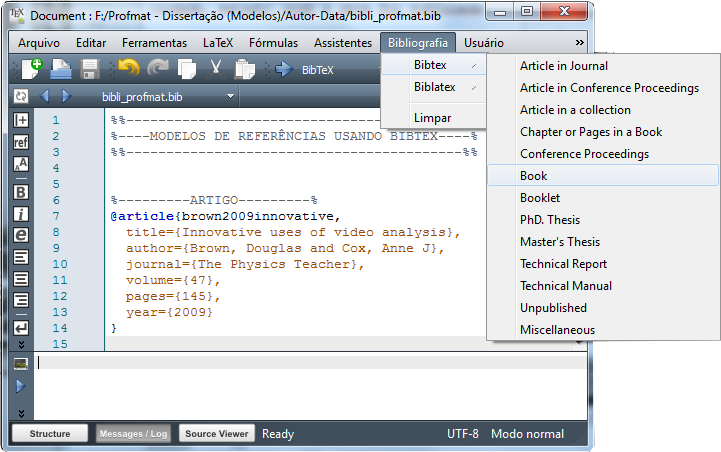
\includegraphics[scale=0.45]
	{img/fig08.png}\label{fig08}\\
	FONTE: Autor (2015)
	\end{figure}


 Como exemplo, observe duas referências escritas no arquivo \textbf{bibliografia.bib}:
\begin{verbatim}
@Manual{nbr14724,
title = {ABNT NBR 14724:2011},
subtitle={Informação
e documentação - trabalhos acadêmicos - apresentação},
author = {ABNT},
address = {Rio de Janeiro},
year = {2011},
}

@Book{AL_hefez,
author = {Abramo Hefez and Cecília de Souza Fernandez},
title = {Introdução à Álgebra Linear},
publisher = {SBM},
series = {Coleção Profmat},
year = {2013},
address = {Rio de Janeiro},
edition = {1},
}
\end{verbatim}

Caso no texto sejam inseridos os comandos \verb!\cite{nbr14724}! e \verb!\cite{AL_hefez}!, uma lista de referências será criada conforme ilustra a figura a seguir:
	\begin{figure}[H]
	\centering
	\caption{Criando referências com bibTeX, resultado em tela}
	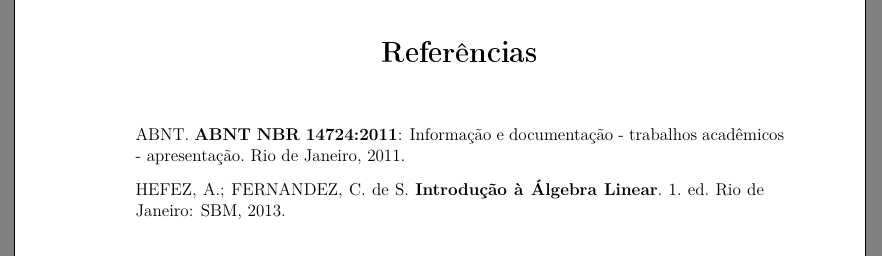
\includegraphics[scale=0.45]
	{img/fig09.png}\label{fig09}\\
	FONTE: Autor (2015)
	\end{figure}


\section{Modelos de citação}

A NBR 10520 define uma citação como uma ``menção de uma informação extraída de outra fonte'' \cite[p.~1]{nbr10520}. A referida norma ainda define os tipos de citação:
\begin{itemize} 
	\item citação direta, quando ocorre a transcrição do texto tal qual está escrino na fonte original;
	\item citação indireta, quando cria-se um texto baseado na obra consultada; e
	\item citação de citação, quando se faz uma citação, direta ou indireta, de um texto ao qual se teve acesso apenas por meio de outro autor,
\end{itemize}
bem como orienta sobre as regras de apresentação das citações no texto.


\subsection{Citação direta}

A norma NBR 10.520 classifica as citações diretas quanto ao tamanho em citações de \textbf{até três linhas} e citações \textbf{com mais de três linhas}. 


\subsubsection{Citação direta com até três linhas}

No caso de citações com \textbf{até três linhas}, as citações ``[$\cdots$] devem estar contidas entre aspas duplas. As aspas simples são
utilizadas para indicar citação no interior da citação'' \cite[p.~2]{nbr10520}. 



A figura abaixo ilustra como escrever em latex uma citação direta com até três linhas:
	\begin{figure}[H]
	\centering
	\caption{Citações com até três linhas}
	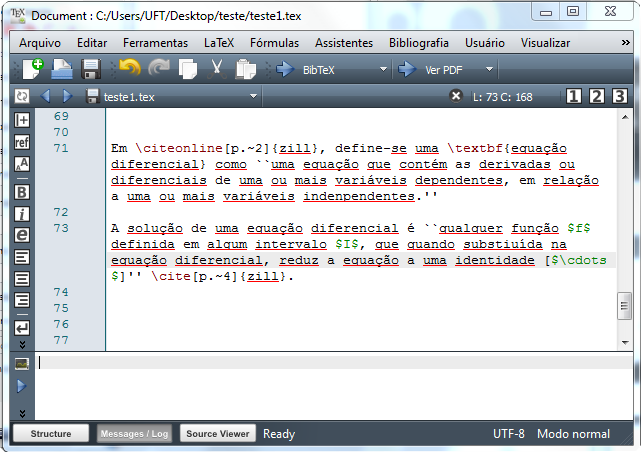
\includegraphics[scale=0.45]
	{img/fig10.png}\label{fig10}\\
	FONTE: Autor (2015)
	\end{figure}

O resultado em PDF é mostrado na Figura \ref{fig11}:
	\begin{figure}[H]
	\centering
	\caption{Citações com até três linhas, resultado em tela}
	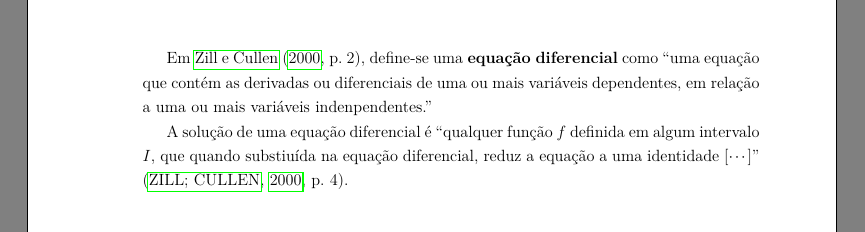
\includegraphics[scale=0.45]
	{img/fig11.png}\label{fig11}\\
	FONTE: Autor (2015)
	\end{figure}
	
	Observe que foram utilizados dois comandos. O comando \verb!\citeonline[]{}! insere a fonte dentro do texto. O nome do autor da fonte aparece com apenas a primeira letra maiúscula. O ano da obra e a página(s) de onde foi retirada a citação estão entre parêntesis. O número da página é inserido na opção \verb![p.~2]!.
	
	O comando \verb!\cite[]{}! insere a fonte, ano da obra e página(s) consultadas entre parêntesis.
	
\subsubsection{Citação direta com mais de três linhas}

Para criar citações com mais de três linhas em LaTeX, é necessário usar o ambiente \texttt{citacao}, conforme exemplo a seguir:
	\begin{figure}[H]
	\centering
	\caption{Citações com mais de três linhas}
	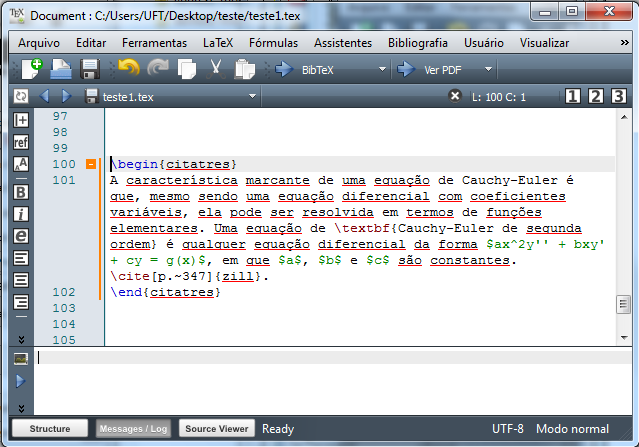
\includegraphics[scale=0.45]
	{img/fig12.png}\label{fig12}\\
	FONTE: Autor (2015)
	\end{figure}
O resultado é mostrado a seguir:
\begin{citacao}
A característica marcante de uma equação de Cauchy-Euler é que, mesmo sendo uma equação diferencial com coeficientes variáveis, ela pode ser resolvida em termos de funções elementares. Uma equação de \textbf{Cauchy-Euler de segunda ordem} é qualquer equação diferencial da forma $ax^2y'' + bxy' + cy = g(x)$, em que $a$, $b$ e $c$ são constantes. \cite[p.~347]{zill}.
\end{citacao}

\subsection{Citação indireta}

As citações indiretas são produzidas em LaTeX utilizando-se os mesmos comandos descritos acima para citação direta com até três linhas. Como exemplo, observe a figura abaixo:
	\begin{figure}[H]
	\centering
	\caption{Citação indireta, comando LaTeX}
	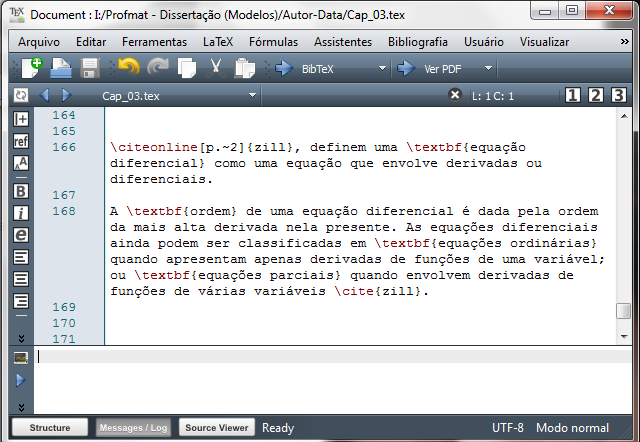
\includegraphics[scale=0.45]
	{img/fig14.png}\label{fig14}\\
	FONTE: Autor (2015)
	\end{figure}

O resultado é mostrado abaixo:
	\begin{figure}[H]
	\centering
	\caption{Citação indireta, em tela}
	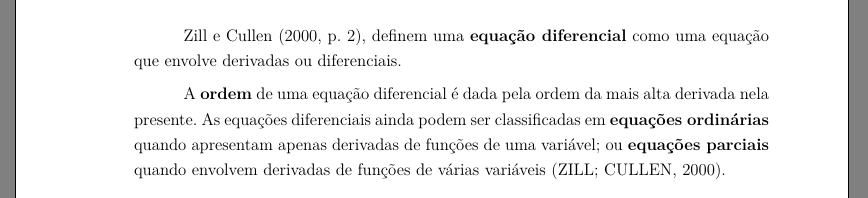
\includegraphics[scale=0.45]
	{img/fig15.png}\label{fig15}\\
	FONTE: Autor (2015)
	\end{figure}
	


\section{Compilando um documento com citações e referências}
 

Para produzir o documento em PDF (para impressão ou leitura em tela do computador), deve-se compilar o código-fonte em LaTeX. Utilizando o editor TexMaker esta ação é realizada clicando no botão \textbf{compilar} na barra de edição do programa conforme ilustra a figura abaixo:
	\begin{figure}[H]
	\centering
	\caption{Compilando o documento LaTeX}
	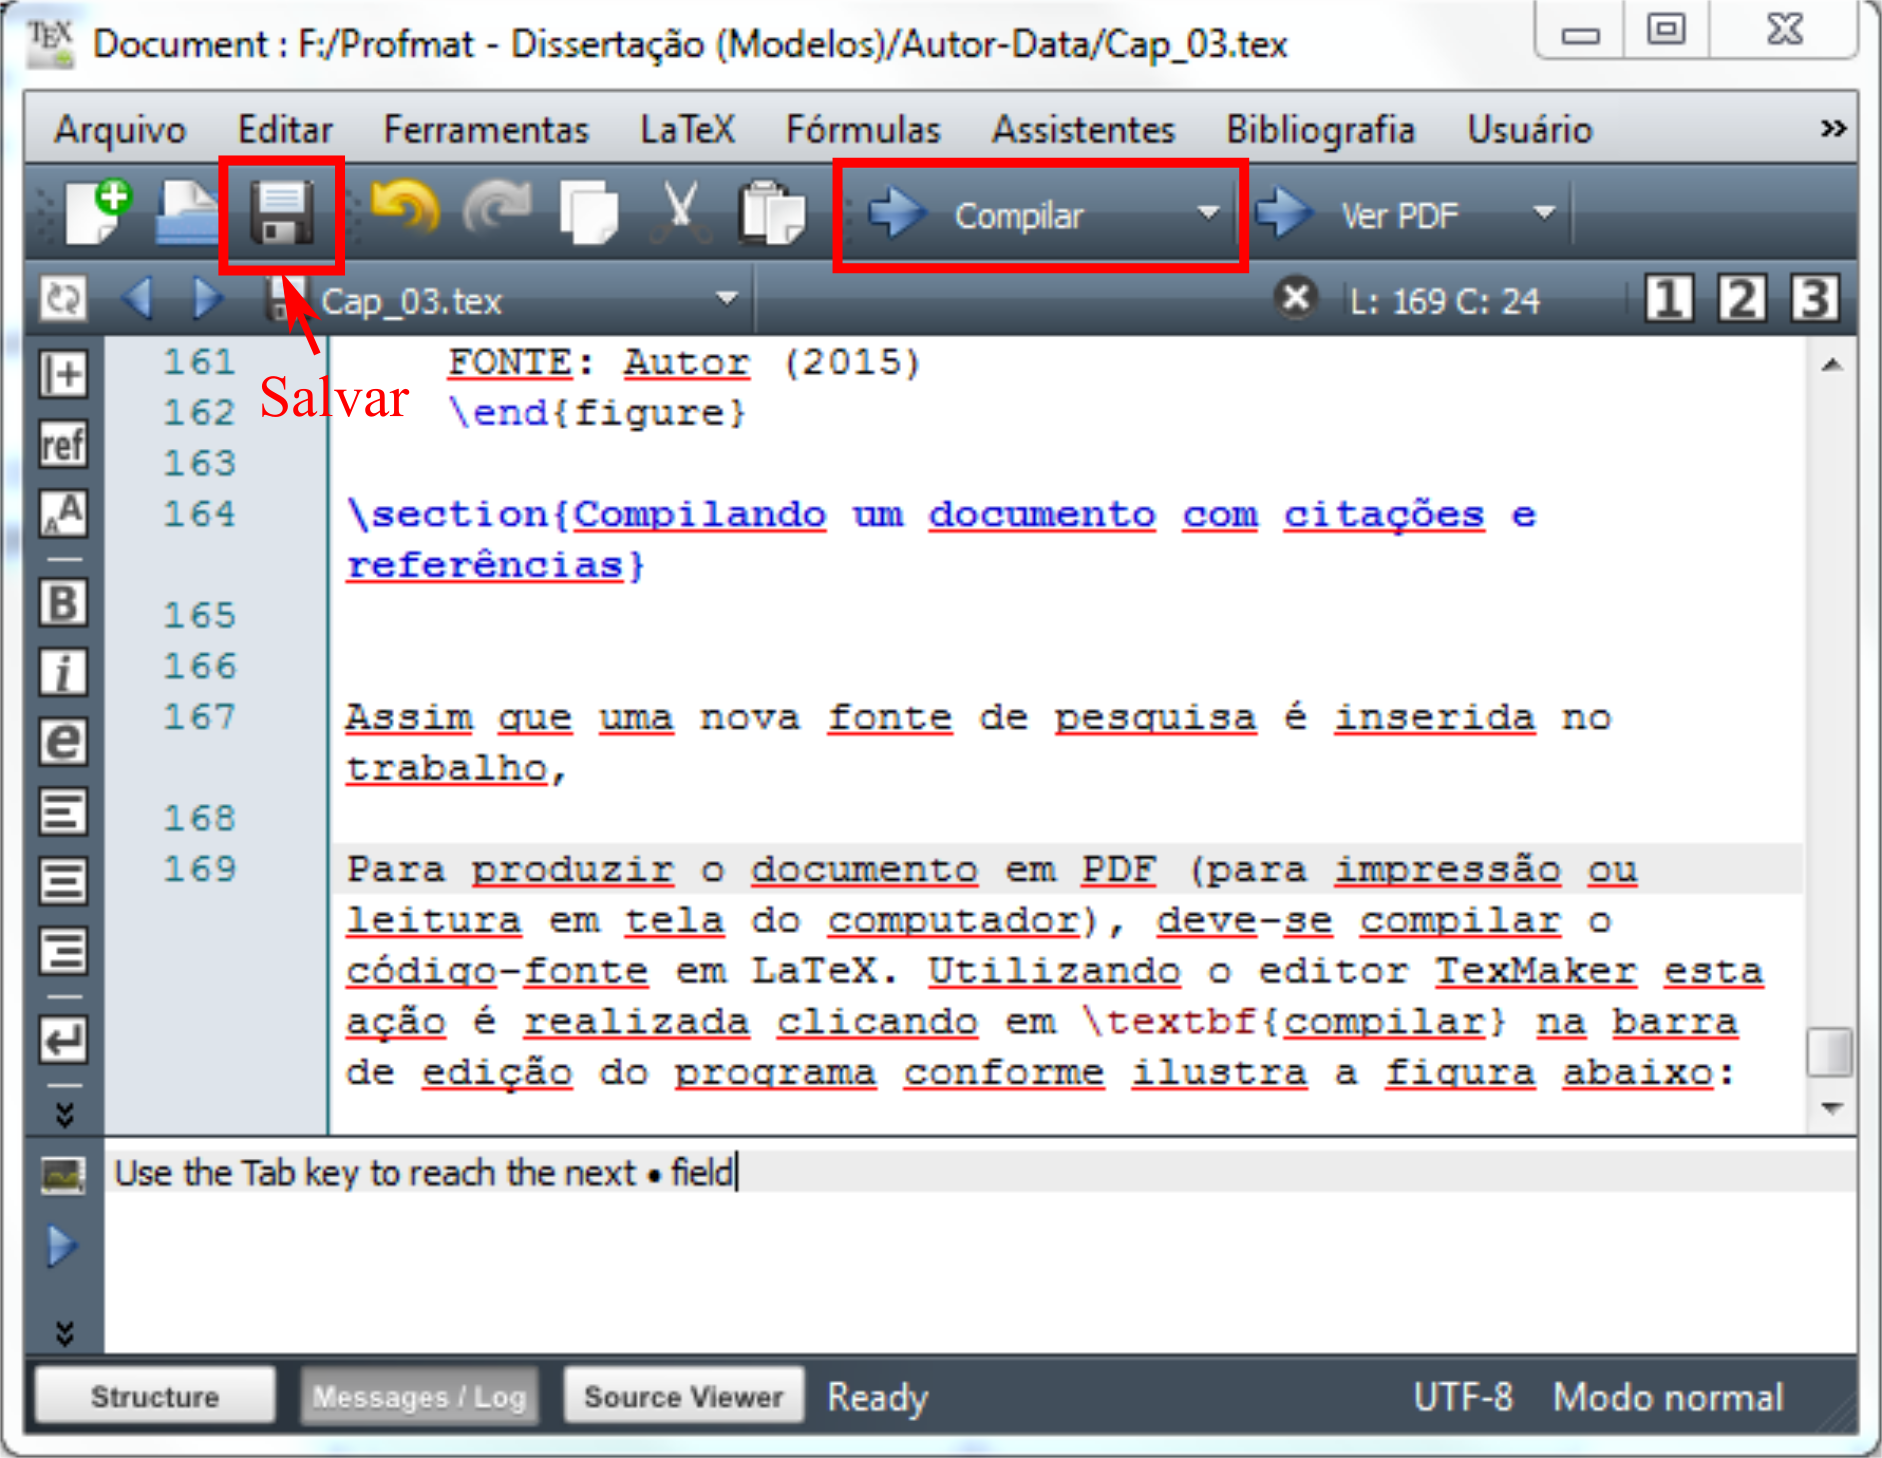
\includegraphics[scale=0.25]
	{img/fig17.png}\label{fig17}\\
	FONTE: Autor (2015)
	\end{figure}
	Uma nova janela será aberta para visualização do resultado em PDF. Na pasta onde o trabalho está sendo salvo, o arquivo \textbf{nome-do-arquivo.pdf} também é atualizado conforme as novas informações inseridas.
	\begin{figure}[H]
	\centering
	\caption{Documento PDF após compilação LaTeX}
	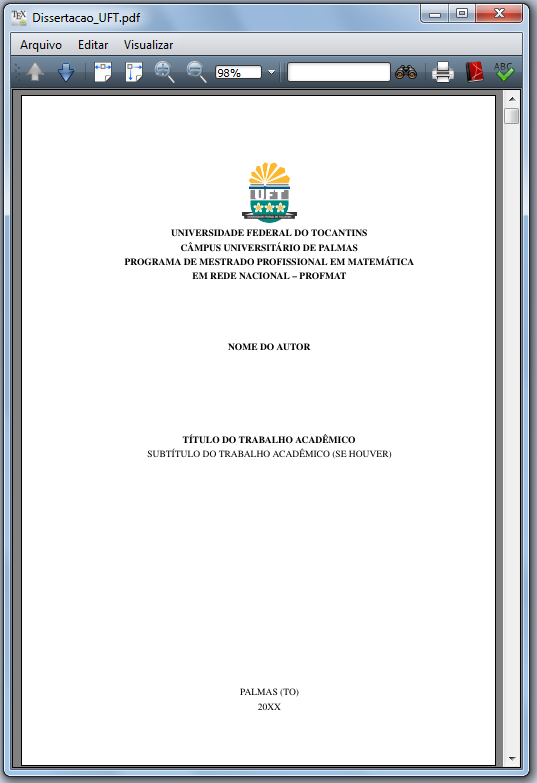
\includegraphics[scale=0.7]
	{img/fig18.png}\label{fig18}\\
	FONTE: Autor (2015)
	\end{figure}
	Neste ponto, uma observação importante. Quando o código-fonte LaTeX está dividido em arquivos menores, como é o caso deste modelo de dissertação, apenas o arquivo mestre (neste modelo, o arquivo \textbf{Dissertacao\_UFT.tex}) deve ser compilado. Os demais arquivos (\textbf{Pretextual.tex}, \textbf{Cap\_01.tex}, \textbf{Cap\_02.tex}, ...) são apenas salvos.
	
	Além disso, assim que uma nova fonte de pesquisa é inserida no trabalho, nem sempre ela aparecerá de imediato no arquivo em PDF. Isso ocorre pois, antes de compilar o código-fonte, é preciso informar ao programa para atualizar o banco de dados bibTeX. Para realizar este procedimento, deve-se clicar na seta ao lado do botão \textbf{compilar}. Aparecerá uma caixa de opções na qual deve-se escolher a opção \textbf{BibTeX}. Após isso, clica-se novamente em \textbf{compilar} para visualizar o arquivo PDF.
	\begin{figure}[H]
	\centering
	\caption{Atualizando banco de dados BibTeX}
	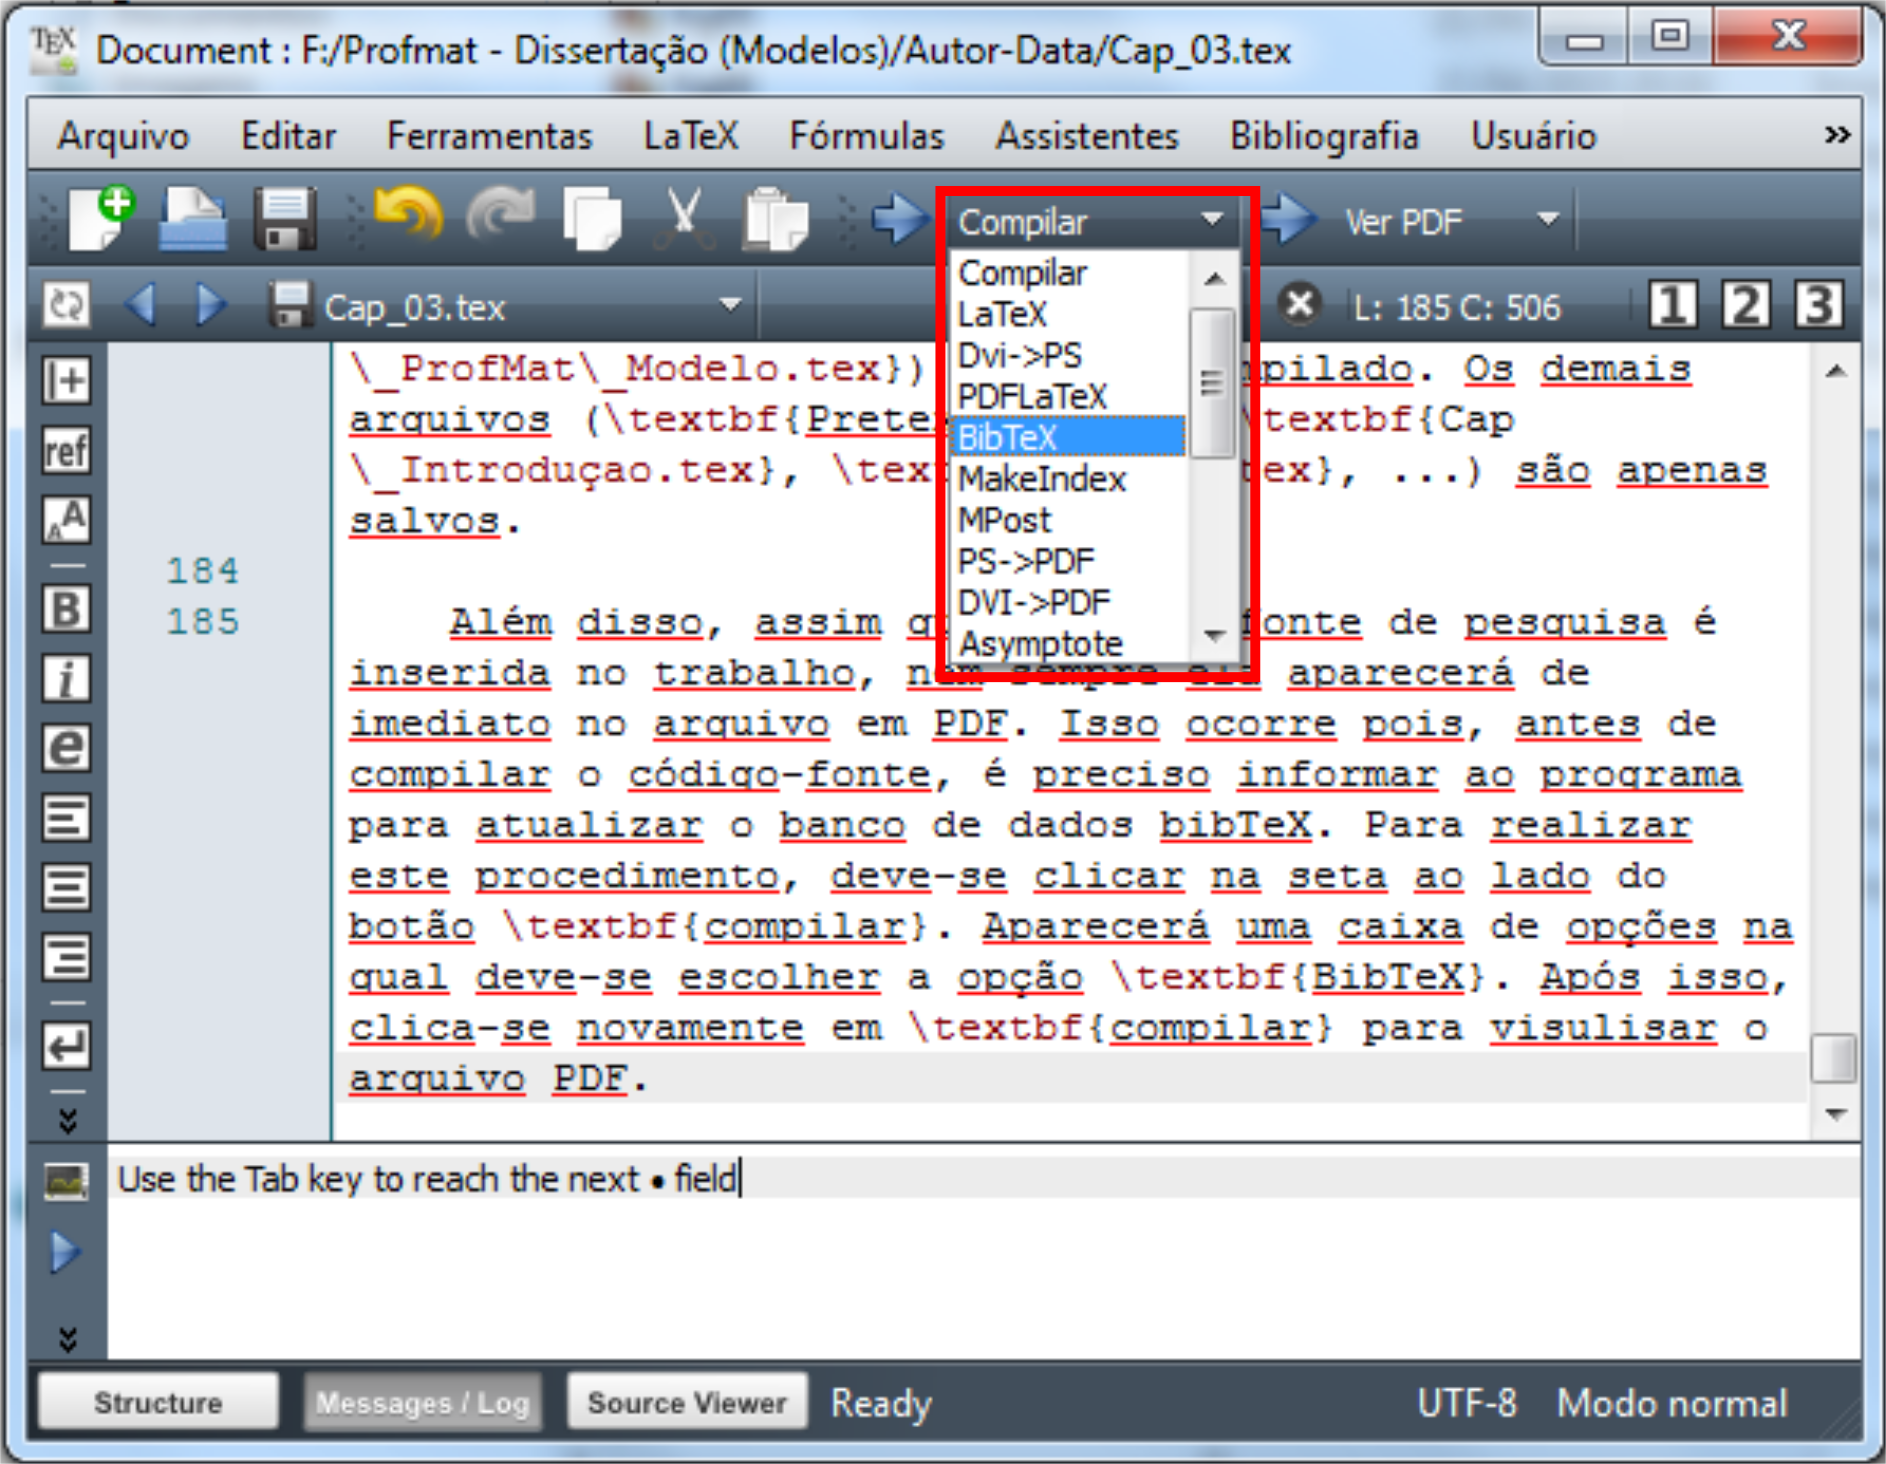
\includegraphics[scale=0.25]
	{img/fig19.png}\label{fig19}\\
	FONTE: Autor (2015)
	\end{figure}
	
	Os procedimentos descritos acima podem ser facilitados e agilizados com o uso de atalhos de teclado. Para um lista completa de atalhos LaTeX no TexMaker, basta clicar em \textbf{Ferramentas} na barra de ferramentas. Para compilar um documento, clique na tecla \keystroke{F1} e para atualizar a lista de referências BibTeX, clique em \keystroke{F11}.
	


%----------------Cap_05----------------%

\chapter{CONCLUSÃO}

Este é o último capítulo da dissertação. Nele, devem ser apresentadas as considerações finais a respeito da pesquisa realizada,  se os objetivos estabelecidos foram alcançados dentre outras informações relevantes.

%--------------------ELEMENTOS PÓS-TEXTUAIS--------------------%

% Abra o arquivo postextual.tex para alterar os elementos pós-textuais de seu trabalho 
%----------------------ELEMENTOS PÓS-TEXTUAIS----------------------%
\postextual

%--------------------Referências Bibliográficas--------------------%
\bibliography{bibliografia}


%-----------------------------Apêndices-----------------------------%
\begin{apendicesenv}

\chapter{Exemplo de apêndice digitado}

O apêndice é escrito como um texto normal da dissertação.

\section*{Regras básicas}

Para que as seções e subsecções  do apêndice não apareçam do sumário, deve-se especificá-las com os comandos:
\begin{verbatim}
\section*{nome-da-seção}
\end{verbatim}

\begin{verbatim}
\subsection*{nome-da-subseção}
\end{verbatim}

O asterisco (\verb!*!) indica ao LaTeX que a seção ou subseção não deve ser adicionada ao sumário.

\subsubsection*{O que é possível}

É possível inserir equações e expressões matemáticas. Por exemplo,
$$\textbf{A} = \left(a_{ij}\right)_{m \times n}$$ 
e  
$$\textbf{B} = \left(b_{ij}\right)_{m \times n}$$ 
são matrizes de mesma ordem...

		\begin{eqnarray*}
		\left\lbrace
		\begin{aligned}
		&a_{11}x_1+a_{12}x_2 + \ldots + a_{1n}x_n = b_1\\
		&a_{21}x_1+a_{22}x_2 + \ldots + a_{2n}x_n = b_2\\
		&\quad \vdots \quad \qquad \qquad \ddots  \quad \qquad \qquad \vdots\\
		&a_{m1}x_1+a_{m2}x_2 + \ldots + a_{mn}x_n = b_m
		\end{aligned}
		\right.
		\end{eqnarray*}
		é um sistema de equações lineares ...
		
	Figuras também são possíveis:
		
	\begin{figure}[H]
	\centering
	\caption{Janela de ajuda do editor TexMaker}
	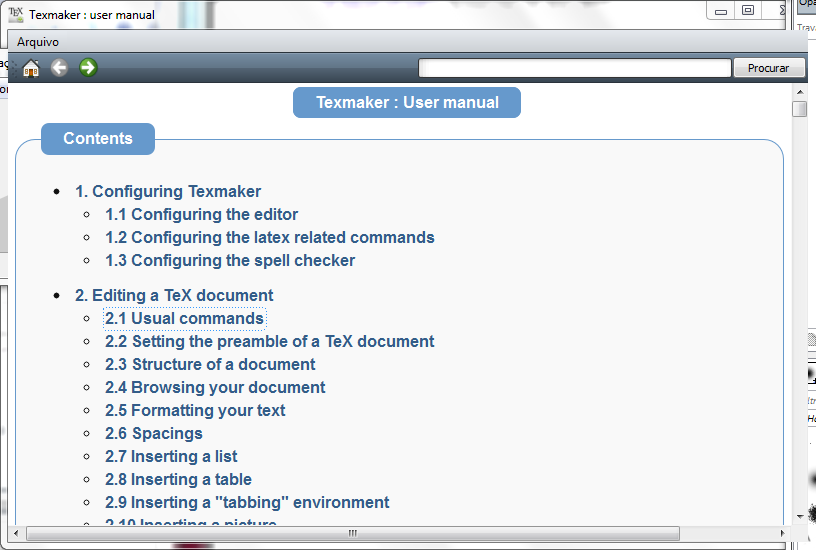
\includegraphics[scale=0.5]
	{img/fig16.png}\label{fig16}\\
	FONTE: Autor (2015)
	\end{figure}

\chapter{Exemplo de apêndice em pdf}
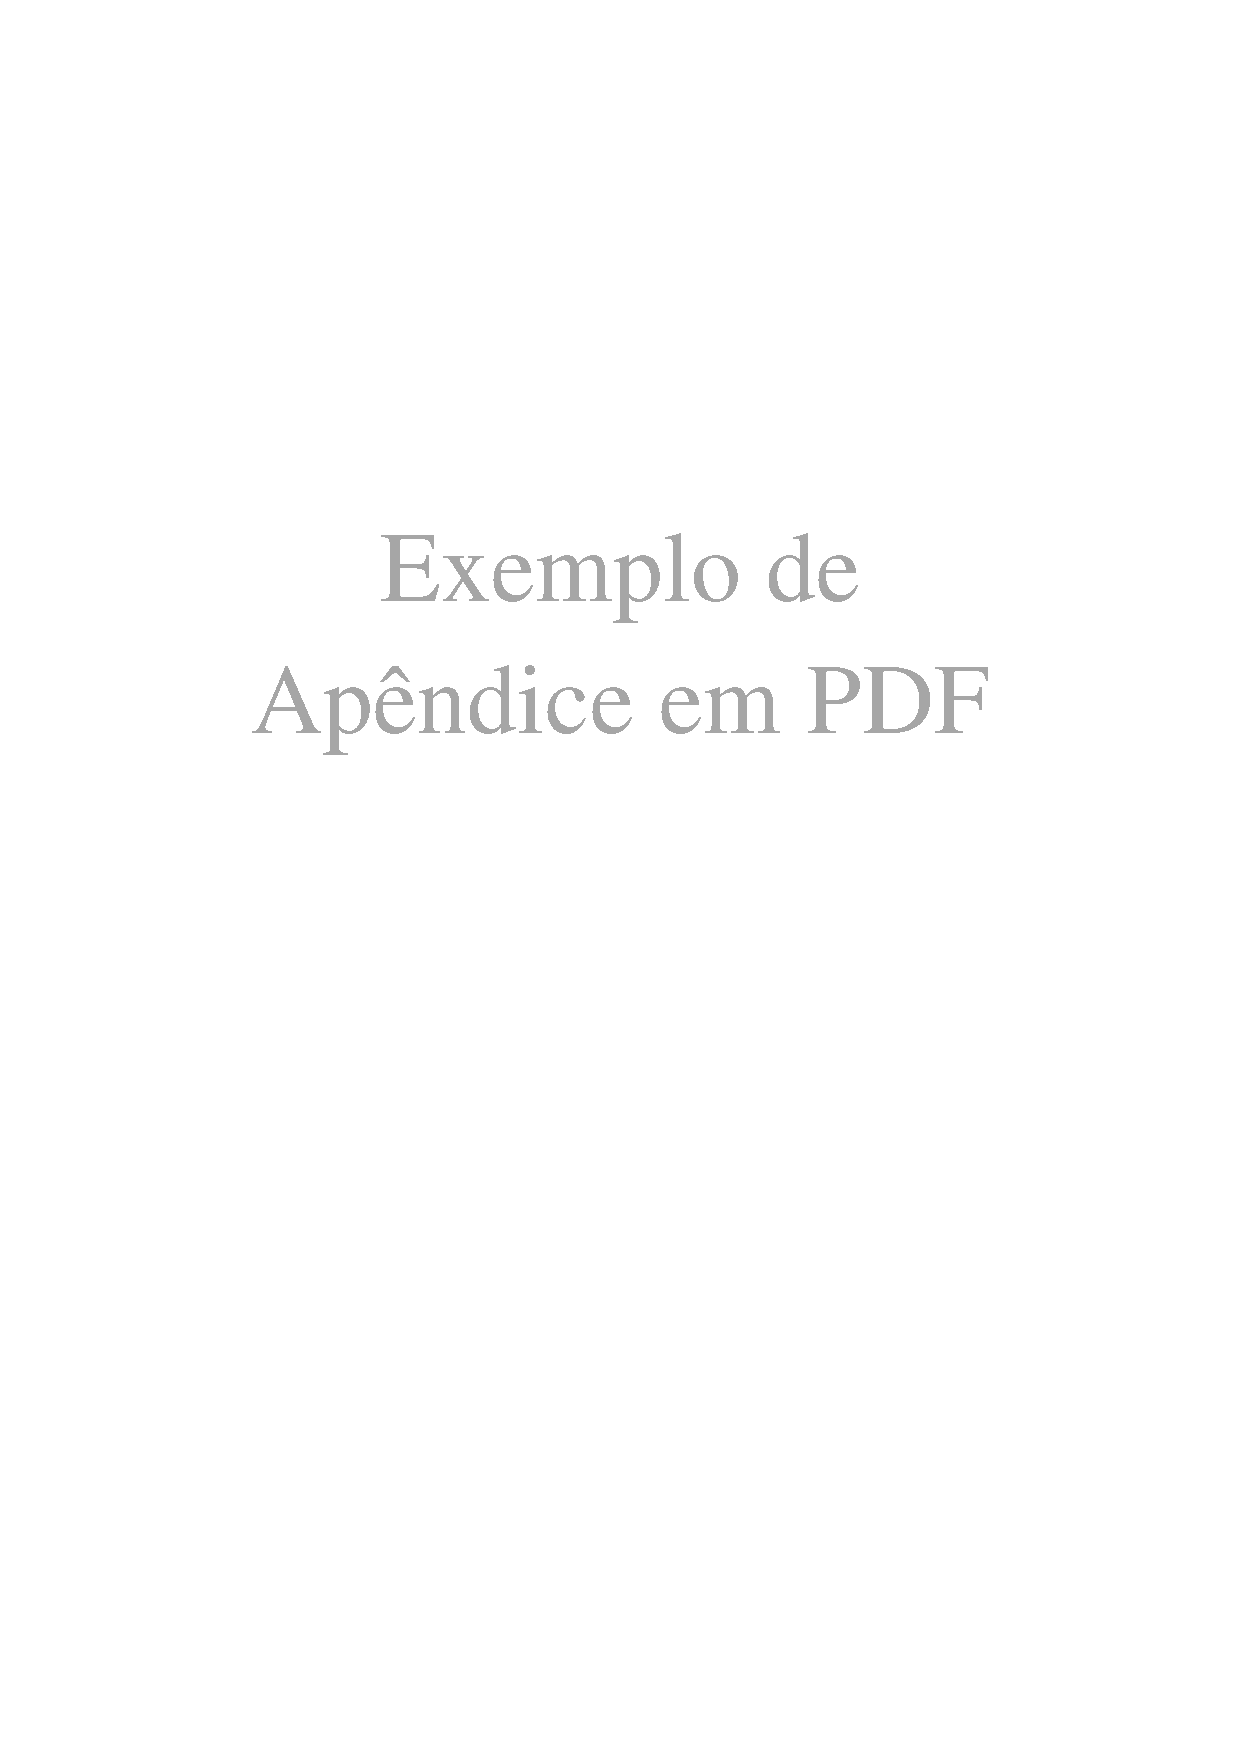
\includepdf[pages=-]{pdf_apendices/apendice_exemplo.pdf}
\end{apendicesenv}

\begin{anexosenv}


%-----------------------------Anexos-----------------------------%
% Imprime uma página indicando o início dos anexos


% ---
\chapter{Exemplo de um anexo digitado}
% ---
\section*{Configuring Texmaker}
Before using Texmaker, you must configure the editor and latex related commands via the ``Configure Texmaker'' command in the ``Options'' menu (``Preferences'' under macosx).
\subsection*{Configuring the editor}

Before compiling your first document, you must set the encoding used by the editor (``Configure Texmaker'' -> ``Editor'' -> ``Editor Font Encoding''). 


% ---
\chapter{Exemplo de anexo em pdf}
% ---
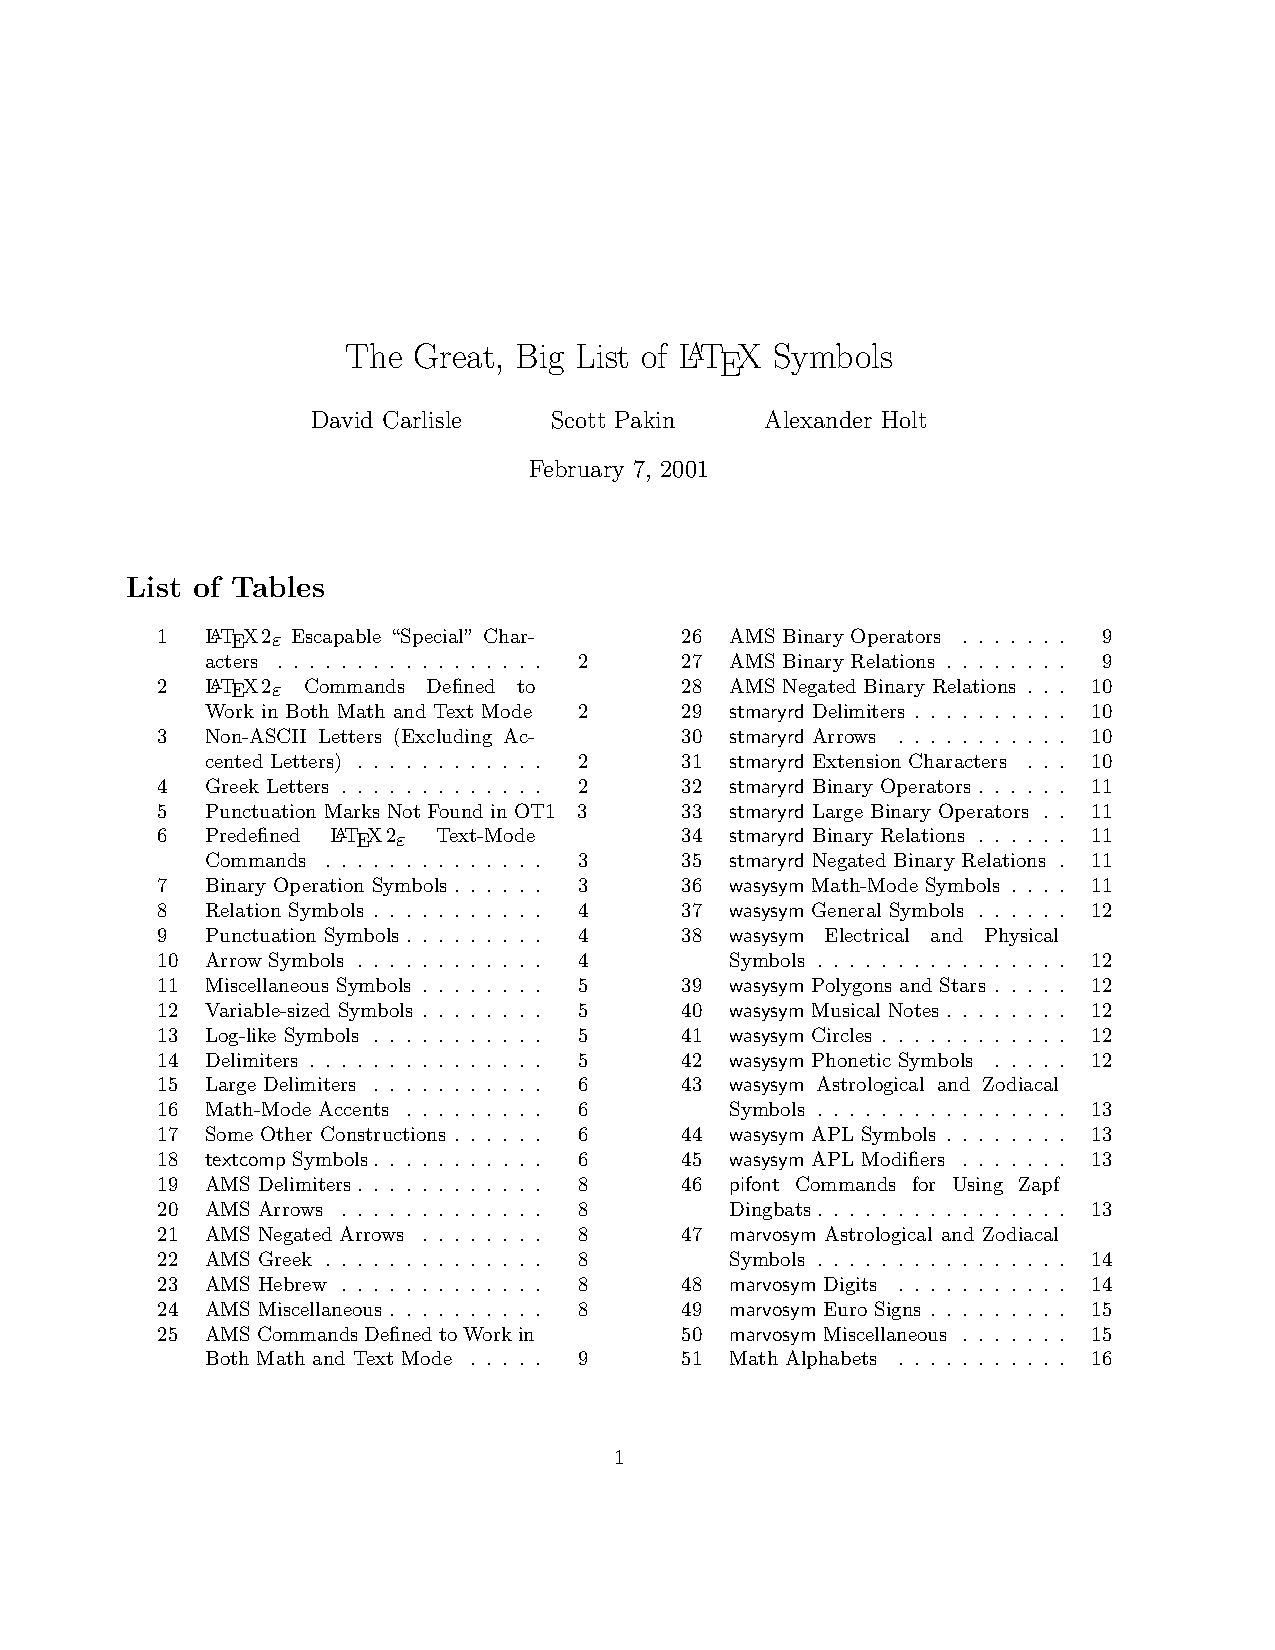
\includepdf[pages=-]{pdf_anexos/anexo_exemplo.pdf}
\end{anexosenv}



\end{document}
%----------------------FIM DA DISSERTAÇÃO----------------------%